% count/count.tex

\QuickQuizChapter{chp:Counting}{Counting}

Counting is perhaps the simplest and most natural for a computer to do.
However, counting efficiently and scalably on a large
shared-memory multiprocessor can be quite challenging.
Furthermore, the simplicity of the underlying concept of counting
allows us to explore the fundamental issues of concurrency without
the distractions
of elaborate data structures or complex synchronization primitives.
Counting therefore provides an excellent introduction to
parallel programming.

This chapter covers a number of special cases for which there are simple,
fast, and scalable counting algorithms.
But first, let us find out how much you already know about concurrent
counting.

\QuickQuiz{}
	Why on earth should efficient and scalable counting be hard???
	After all, computers have special hardware for the sole purpose
	of doing counting,
	addition, subtraction, and lots more besides, don't they???
\QuickQuizAnswer{
	Because the straightforward counting algorithms, for example,
	atomic operations on a shared counter, are slow and scale
	badly, as will be seen in
	Section~\ref{sec:count:Why Isn't Concurrent Counting Trivial?}.
} \QuickQuizEnd

\QuickQuiz{}
	Suppose that you need to collect statistics on the number
	of networking packets (or total number of bytes) transmitted
	and/or received.
	Packets might be transmitted or received by any CPU on
	the system.
	Suppose further that this large machine is capable of
	handling a million packets per second, and that there
	is a systems-monitoring package that reads out the count
	every five seconds.
	How would you implement this statistical counter?
\QuickQuizAnswer{
	Hint: the act of updating the counter must be blazingly
	fast, but because the counter is read out only about once
	in five million updates, the act of reading out the counter can be
	quite slow.
	In addition, the value read out normally need not be all that
	accurate---after all, since the counter is updated a thousand
	times per millisecond, we should be able to work with a value
	that is within a few thousand counts of the ``true value'',
	whatever ``true value'' might mean in this context.
	However, the value read out should maintain roughly the same
	absolute error over time.
	For example, a 1\% error might be just fine when the count
	is on the order of a million or so, but might be absolutely
	unacceptable once the count reaches a trillion.
	See Section~\ref{sec:count:Statistical Counters}.
} \QuickQuizEnd

\QuickQuiz{}
	Suppose that you need to maintain a count of the number of
	structures allocated in order to fail any allocations
	once the number of structures in use exceeds a limit
	(say, 10,000).
	Suppose further that these structures are short-lived,
	and that the limit is rarely exceeded.
\QuickQuizAnswer{
	Hint: the act of updating the counter must be blazingly
	fast, but the counter is read out each time that the
	counter is increased.
	However, the value read out need not be accurate
	\emph{except} that it absolutely must distinguish perfectly
	between values below the limit and values greater than or
	equal to the limit.
	See Section~\ref{sec:count:Limit Counters}.
} \QuickQuizEnd

\QuickQuiz{}
	Suppose that you need to maintain a count of the number of
	structures allocated in order to fail any allocations
	once the number of structures in use exceeds a limit
	(say, 10,000).
	Suppose further that these structures are short-lived,
	and that the limit is rarely exceeded, that there is almost
	always at least one structure in use, and suppose further
	still that it is necessary to know when this counter reaches
	zero, for example, in order to free up some memory
	that is not required unless there is at least one structure
	in use.
\QuickQuizAnswer{
	Hint: the act of updating the counter must be blazingly
	fast, but the counter is read out each time that the
	counter is increased.
	However, the value read out need not be accurate
	\emph{except} that it absolutely must distinguish perfectly
	between values between the limit and zero on the one hand,
	and values that either are less than or equal to zero or
	are greater than or equal to the limit on the other hand.
	See Section~\ref{sec:count:Double-Limit Counters}.
} \QuickQuizEnd

\QuickQuiz{}
	Suppose that you need to maintain a reference count on a
	heavily used removable mass-storage device, so that you
	can tell the user when it is safe to removed the device.
	This device follows the usual removal procedure where
	the user indicates a desire to remove the device, and
	the system tells the user when it is safe to do so.
\QuickQuizAnswer{
	Hint: the act of updating the counter must be blazingly
	fast, but because the counter is read out only when the
	user wishes to remove the device, the counter read-out
	operation can be extremely slow.
	Furthermore, there is no need to be able to read out
	the counter at all unless the user has already indicated
	a desire to remove the device.
	In addition, the value read out need not be accurate
	\emph{except} that it absolutely must distinguish perfectly
	between non-zero and zero values.
	However, once it has read out a zero value, it must act
	to keep the value at zero until it has taken some action
	to prevent subsequent threads from gaining access to the
	device being removed.
	See Section~\ref{sec:count:Atomic-Read Reference Counters}.
} \QuickQuizEnd

The remainder of this chapter will develop answers to these questions.

\section{Why Isn't Concurrent Counting Trivial?}
\label{sec:count:Why Isn't Concurrent Counting Trivial?}

\begin{figure}[bp]
{ \scriptsize
\begin{verbatim}
  1 long counter = 0;
  2 
  3 void inc_count(void)
  4 {
  5   counter++;
  6 }
  7 
  8 long read_count(void)
  9 {
 10   return counter;
 11 }
\end{verbatim}
}
\caption{Just Count!}
\label{fig:count:Just Count!}
\end{figure}

Let's start with something simple, for example, the straightforward
use of arithmetic shown in
Figure~\ref{fig:count:Just Count!} (\url{count_nonatomic.c}).
Here, we have a counter on line~1, we increment it on line~5, and we
read out its vale on line~10.
What could be simpler?

This approach has the additional advantage of being blazingly fast if
you are doing lots of reading and almost no incrementing, and on small
systems, the increment speed is also pretty good.

There is just one large fly in the ointment: this approach can lose
counts.
On my dual-core laptop, a short run invoked \url{inc_count()}
100,014,000 times, but the final value of the counter was only
52,909,118.
Although it is true that approximate values have their place in computing,
this result is off by almost a factor of two!!!

\QuickQuiz{}
	But doesn't the \url{++} operator produce an x86 add-to-memory
	instruction?
	And won't the CPU cache cause this to be atomic?
\QuickQuizAnswer{
	Although the \url{++} operator \emph{could} be atomic, there
	is no requirement that it be so.
	Furthermore, the \url{ACCESS_ONCE()} primitive forces most
	version of \url{gcc} to load the value to a register, increment
	the register, then store the value to memory, which is
	decidedly non-atomic.
} \QuickQuizEnd

\begin{figure}[bp]
{ \scriptsize
\begin{verbatim}
  1 atomic_t counter = ATOMIC_INIT(0);
  2 
  3 void inc_count(void)
  4 {
  5   atomic_inc(&counter);
  6 }
  7 
  8 long read_count(void)
  9 {
 10   return atomic_read(&counter);
 11 }
\end{verbatim}
}
\caption{Just Count Atomically!}
\label{fig:count:Just Count Atomically!}
\end{figure}

\begin{figure}[tb]
\begin{center}
\resizebox{3in}{!}{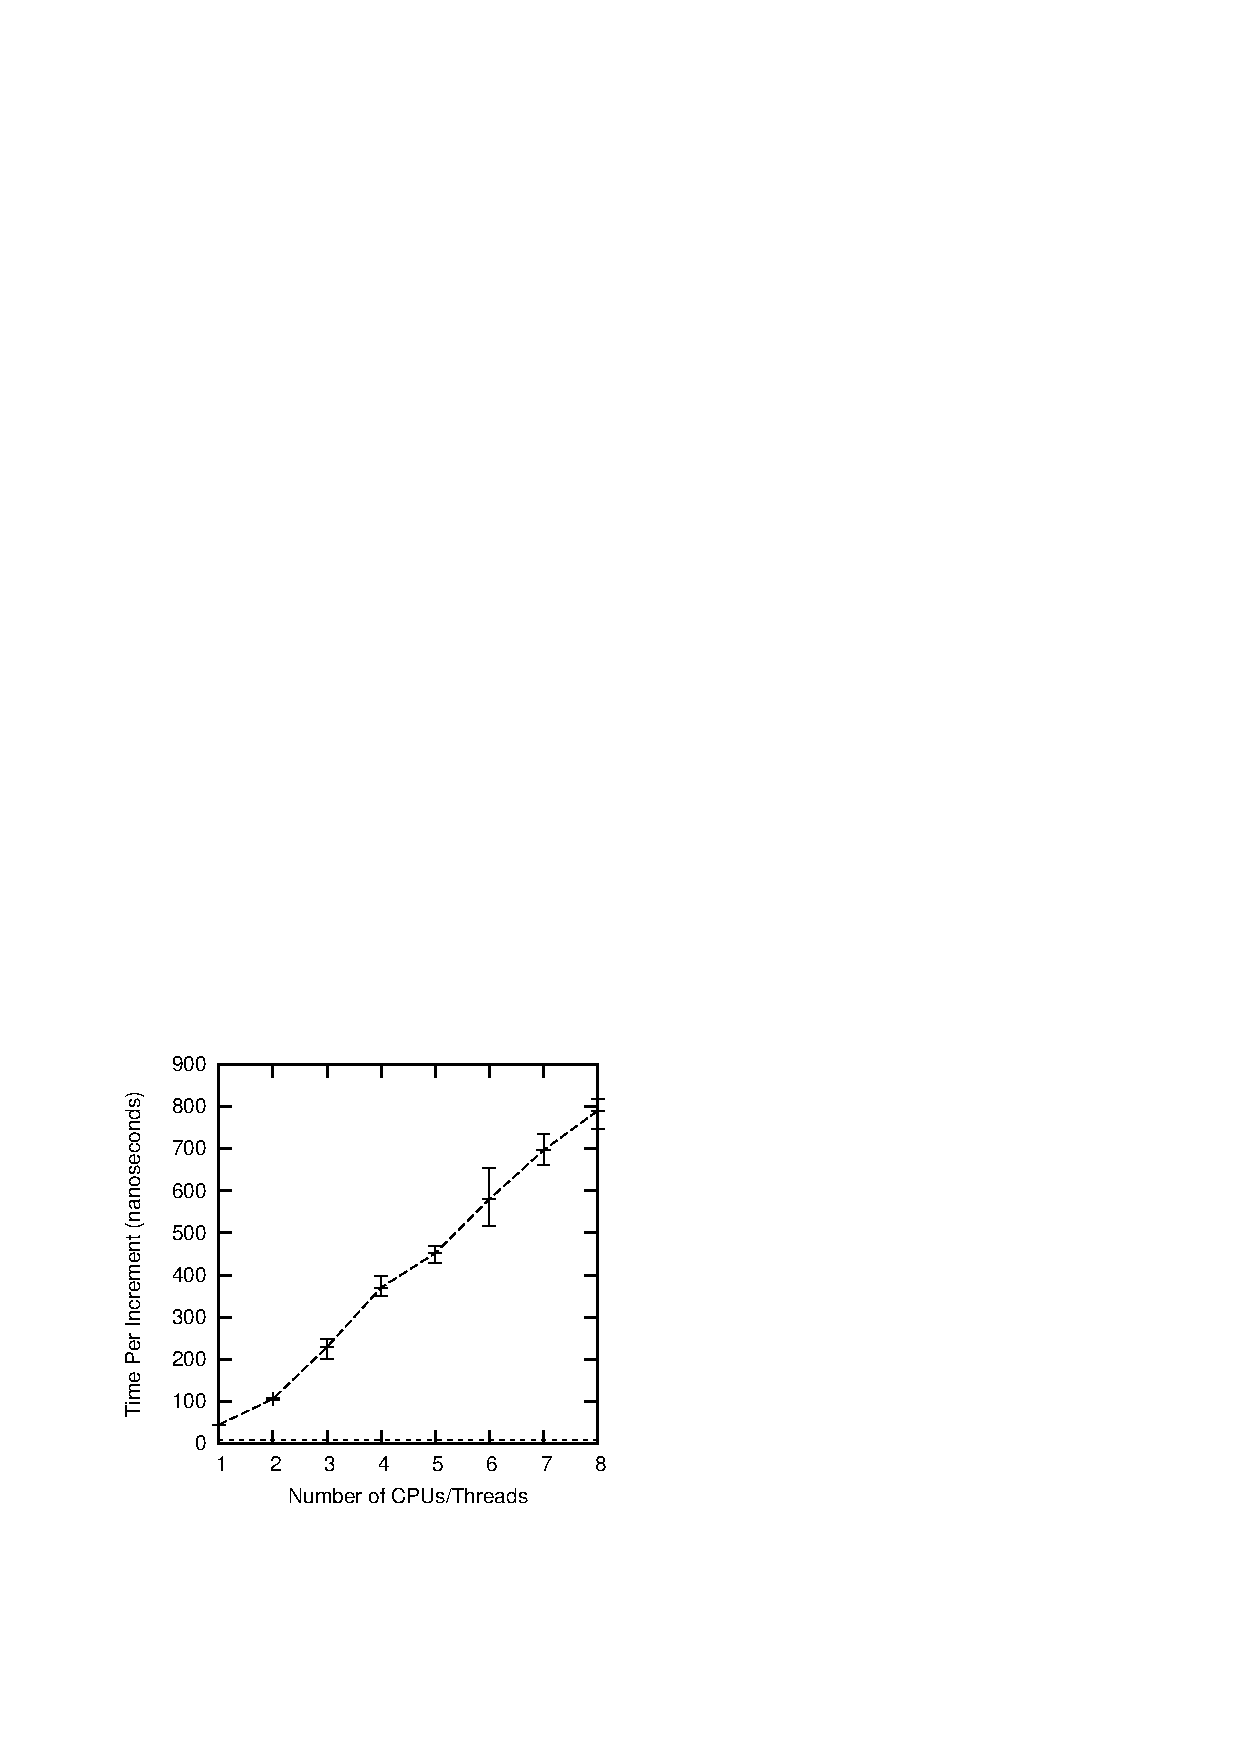
\includegraphics{CodeSamples/count/atomic}}
\end{center}
\caption{Atomic Increment Scalability on Nehalem}
\label{fig:count:Atomic Increment Scalability on Nehalem}
\end{figure}

The straightforward way to count accurately is to use atomic operations,
as shown in
Figure~\ref{fig:count:Just Count Atomically!} (\url{count_atomic.c}).
Line~1 defines an atomic variable, line~5 atomically increments it, and
line~10 reads it out.
Because this is atomic, it keeps perfect count.
However, it is slower: on a Intel Core Duo laptop, it is about
six times slower than non-atomic increment
when a single thread is incrementing, and more than \emph{ten times}
slower if two threads are incrementing.

This poor performance should not be a surprise, given the discussion in
Chapter~\ref{chp:Hardware and its Habits},
nor should it be a surprise that the performance of atomic increment
gets slower as the number of CPUs and threads increase, as shown in
Figure~\ref{fig:count:Atomic Increment Scalability on Nehalem}.
In this figure, the horizontal dashed line resting on the x~axis
is the ideal performance that would be achieved
by a perfectly scalable algorithm: with such an algorithm, a given
increment would incur the same overhead that it would in a single-threaded
program.
Atomic increment of a single global variable is clearly
decidedly non-ideal, and gets worse as you add CPUs.

\QuickQuiz{}
	Why doesn't the dashed line on the x~axis meet the 
	diagonal line at $y=1$?
\QuickQuizAnswer{
	Because of the overhead of the atomic operation.
	The dashed line on the x~axis represents the overhead of
	a single \emph{non-atomic} increment.
	After all, an \emph{ideal} algorithm would not only scale
	linearly, it would also incur no performance penalty compared
	to single-threaded code.

	This level of ideality may seem severe, but if it is good
	enough for Linus Torvalds, it is good enough for you.
} \QuickQuizEnd

\QuickQuiz{}
	But atomic increment is still pretty fast.
	And incrementing a single variable in a tight loop sounds
	pretty unrealistic to me, after all, most of the program's
	execution should be devoted to actually doing work, not accounting
	for the work it has done!
	Why should I care about making this go faster?
\QuickQuizAnswer{
	In many cases, atomic increment will in fact be fast enough
	for you.
	In those cases, you should by all means use atomic increment.
	That said, there are many real-world situations where
	more elaborate counting algorithms are required.
	The canonical example of such a situation is counting packets
	and bytes in highly optimized networking stacks, where it is
	all too easy to find much of the execution time going into
	these sorts of accounting tasks, especially on large
	multiprocessors.

	In addition, counting provides an excellent view of the
	issues encountered in shared-memory parallel programs.
} \QuickQuizEnd

\begin{figure}[tb]
\begin{center}
\resizebox{3in}{!}{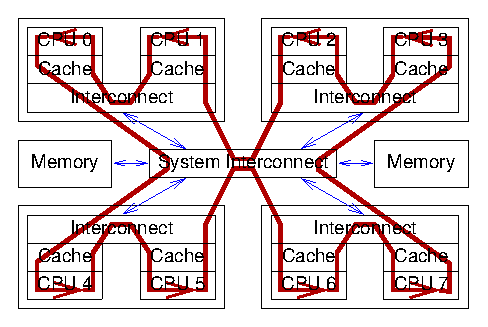
\includegraphics{count/GlobalInc}}
\end{center}
\caption{Data Flow For Global Atomic Increment}
\label{fig:count:Data Flow For Global Atomic Increment}
\end{figure}

For another perspective on global atomic increment, consider
Figure~\ref{fig:count:Data Flow For Global Atomic Increment}.
In order for each CPU to get a chance to increment a given
global variable, the cache line containing that variable must
circulate among all the CPUs, as shows by the red arrows.
Such circulation will take significant time, resulting in
the poor performance seen in
Figure~\ref{fig:count:Atomic Increment Scalability on Nehalem}.

The following sections discuss high-performance counting, which
avoids the delays inherent in such circulation.

\QuickQuiz{}
	But why can't CPU designers simply ship the operation to the
	data, avoiding the need to circulate the cache line containing
	the global variable being incremented?
\QuickQuizAnswer{
	It might well be possible to do this in some cases.
	However, there are a few complications:
	\begin{enumerate}
	\item	If the value of the variable is required, then the
		thread will be forced to wait for the the operation
		to be shipped to the data, and then for the result
		to be shipped back.
	\item	If the atomic increment must be ordered with respect
		to prior and/or subsequent operations, then the thread
		will be forced to wait for the operation to be shipped
		to the data, and for an indication that the operation
		completed to be shipped back.
	\item	Shipping operations among CPUs will likely require
		more signals, which will consume more die area and
		more electrical power.
	\end{enumerate}
	But what if neither of the first two conditions holds?
	Then you should think carefully about the algorithms discussed
	in Section~\ref{sec:count:Statistical Counters}, which achieve
	near-ideal performance on commodity hardware.

\begin{figure}[tb]
\begin{center}
\resizebox{3in}{!}{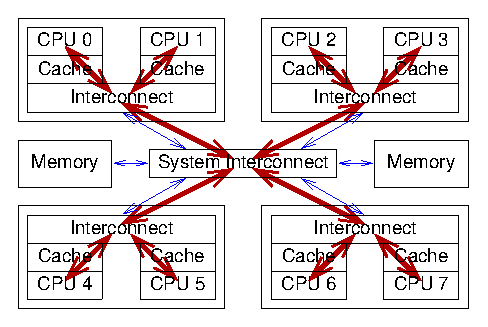
\includegraphics{count/GlobalTreeInc}}
\end{center}
\caption{Data Flow For Global Combining-Tree Atomic Increment}
\label{fig:count:Data Flow For Global Combining-Tree Atomic Increment}
\end{figure}

	If either or both of the first two conditions hold, there is
	\emph{some} hope for improvement.
	One could imagine the hardware implementing a combining tree,
	so that the increment requests from multiple CPUs are combined
	by the hardware into a single addition when the combined request
	reaches the hardware.
	The hardware could also apply an order to the requests, thus
	returning to each CPU the return value corresponding to its
	particular atomic increment.
	This results in instruction latency that varies as $O(log N)$,
	where $N$ is the number of CPUs, as shown in
	Figure~\ref{fig:count:Data Flow For Global Combining-Tree Atomic Increment}.

	Although this is a great improvement over the $O(N)$ performance
	of current hardware shown in
	Figure~\ref{fig:count:Data Flow For Global Atomic Increment},
	we will see that in some important special cases, software
	can do much better.
} \QuickQuizEnd

\section{Statistical Counters}
\label{sec:count:Statistical Counters}

One common special case of counting is statistical counters, where
the count is updated extremely frequently and the value is read out
rarely, if ever.
This situation is typically handled by providing a counter per
thread (or CPU, when running in the kernel), so that each thread
updates its counter.
To read out the aggregate value of the counters, simply sum up
all the threads' counters.

\begin{figure}[bp]
{ \scriptsize
\begin{verbatim}
  1 DEFINE_PER_THREAD(long, counter);
  2 
  3 void inc_count(void)
  4 {
  5   __get_thread_var(counter)++;
  6 }
  7 
  8 long read_count(void)
  9 {
 10   int t;
 11   long sum = 0;
 12 
 13   for_each_thread(t)
 14     sum += per_thread(counter, t);
 15   return sum;
 16 }
\end{verbatim}
}
\caption{Array-Based Per-Thread Statistical Counters}
\label{fig:count:Array-Based Per-Thread Statistical Counters}
\end{figure}

One way to do this is to allocate an array with one element per
thread (presumably cache aligned and padded to avoid false sharing).
Such an array can be wrapped into per-thread primitives, as shown in
Figure~\ref{fig:count:Array-Based Per-Thread Statistical Counters}
(\url{count_stat.c}).
Line~1 defines an array containing a set of per-thread counters of
type \url{long} named, creatively enough, \url{counter}.

Lines~3-6 show a function that increments the counters, using the
\url{__get_thread_var()} primitive to locate the currently running
thread's element of the \url{counter} array.
Because this element is modified only by the corresponding thread,
non-atomic increment suffices.

Lines~8-16 show a function that reads out the aggregate value of the counter,
using the \url{for_each_thread()} primitive to iterate over the list of
currently running threads, and using the \url{per_thread()} primitive
to fetch the specified thread's counter.
Because the hardware can fetch and store a properly aligned \url{long}
atomically, and because gcc is kind enough to make use of this capability,
normal loads suffice, and no special atomic instructions are required.

\QuickQuiz{}
	What other choice does gcc have, anyway???
\QuickQuizAnswer{
	According to the C standard, the effects of fetching a variable
	that might be concurrently modified by some other thread are
	undefined.
	It turns out that the C standard really has no other choice,
	given that C must support (for example) eight-bit architectures
	which are incapable of atomically loading a \url{long}.
	An upcoming version of the C standard aims to fill this gap,
	but until then, we depend on the kindness of the gcc developers.
} \QuickQuizEnd

\begin{figure}[tb]
\begin{center}
\resizebox{3in}{!}{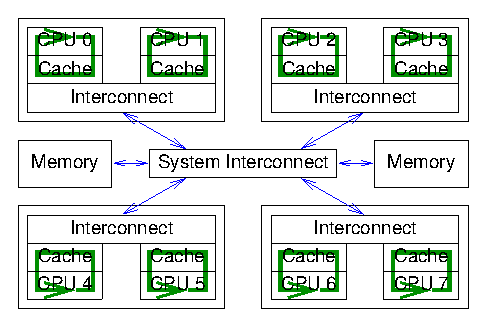
\includegraphics{count/PerThreadInc}}
\end{center}
\caption{Data Flow For Per-Thread Increment}
\label{fig:count:Data Flow For Per-Thread Increment}
\end{figure}

This approach scales linearly with increasing number of updater threads
invoking \url{inc_count()}.
As is shows by the green arrows in
Figure~\ref{fig:count:Data Flow For Per-Thread Increment},
the reason for this is that each CPU can make rapid progress incrementing
its thread's variable, with no expensive communication required crossing
the full diameter of the computer system.
However, this excellent scalability comes at the cost of increased
overhead compared to that of the simple non-atomic increment.
This overhead is due to the array indexing hidden in the
\url{__get_thread_var()} primitive.

\begin{figure}[bp]
{ \scriptsize
\begin{verbatim}
  1 long __thread counter = 0;
  2 long *counterp[NR_THREADS] = { NULL };
  3 long finalcount = 0;
  4 DEFINE_SPINLOCK(final_mutex);
  5 
  6 void inc_count(void)
  7 {
  8   counter++;
  9 }
 10 
 11 long read_count(void)
 12 {
 13   int t;
 14   long sum;
 15 
 16   spin_lock(&final_mutex);
 17   sum = finalcount;
 18   for_each_thread(t)
 19     if (counterp[t] != NULL)
 20       sum += *counterp[t];
 21   spin_unlock(&final_mutex);
 22   return sum;
 23 }
 24 
 25 void count_register_thread(void)
 26 {
 27   int idx = smp_thread_id();
 28 
 29   spin_lock(&final_mutex);
 30   counterp[idx] = &counter;
 31   spin_unlock(&final_mutex);
 32 }
 33 
 34 void count_unregister_thread(int nthreadsexpected)
 35 {
 36   int idx = smp_thread_id();
 37 
 38   spin_lock(&final_mutex);
 39   finalcount += counter;
 40   counterp[idx] = NULL;
 41   spin_unlock(&final_mutex);
 42 }
\end{verbatim}
}
\caption{Per-Thread Statistical Counters}
\label{fig:count:Per-Thread Statistical Counters}
\end{figure}

Fortunately, gcc provides an \url{__thread} storage class that provides
per-thread storage.
This can be used as shown in
Figure~\ref{fig:count:Per-Thread Statistical Counters} (\url{count_end.c})
to implement
a statistical counter that not only scales, but that also incurs little
or no performance penalty to incrementers compared to simple non-atomic
increment.

Lines~1-4 define needed variables: \url{counter} is the per-thread counter
variable, the \url{counterp[]} array allows threads to access each others'
counters, finalcount accumulates the total as individual threads exit,
and \url{final_mutex} coordinates between threads accumulating the total
value of the counter and exiting threads.

\QuickQuiz{}
	Why do we need an explicit array to find the other threads'
	counters?
	Why doesn't gcc provide a \url{per_thread()} interface, similar
	to the Linux kernel's \url{per_cpu()} primitive, to allow
	threads to more easily access each others' per-thread variables?
\QuickQuizAnswer{
	Why indeed?

	To be fair, gcc faces some challenges that the Linux kernel
	gets to ignore.
	When a user-level thread exits, its per-thread variables all
	disappear, which complicates the problem of per-thread-variable
	access, particularly before the advent of user-level RCU.
	In contrast, in the Linux kernel, when a CPU goes offline,
	that CPU's per-CPU variables remain mapped and accessible.

	Similarly, when a new user-level thread is created, its
	per-thread variables suddenly come into existence.
	In contrast, in the Linux kernel, all per-CPU variables are
	mapped and initialized at boot time, regardless of whether
	the corresponding CPU exists yet, or indeed, whether the
	corresponding CPU will ever exist.

	A key limitation that the Linux kernel imposes is a compile-time
	maximum limit on the number of CPUs, namely,
	\url{CONFIG_NR_CPUS}.
	In contrast, in user space, there is no hard-coded upper limit
	on the number of threads.

	Of course, both environments must deal with dyanmically loaded
	code (dynamic libraries in user space, kernel modules in the
	Linux kernel), which increases the complexity of per-thread
	variables in both environments.

	These complications make it significantly harder for user-space
	environments to provide access to other threads' per-thread
	variables.
	Nevertheless, such access is highly useful, and it is hoped
	that it will someday appear.
} \QuickQuizEnd

The \url{inc_count()} function used by updaters is quite simple, as can
be seen on lines~6-9.

The \url{read_count()} function used by readers is a bit more complex.
Line~16 acquires a lock to exclude exiting threads, and line~21 releases
it.
Line~17 initializes the sum to the count accumulated by those threads that
have already exited, and lines~18-20 sum the counts being accumulated
by threads currently running.
Finally, line~22 returns the sum.

\QuickQuiz{}
	Why on earth do we need something as heavyweight as a \emph{lock}
	guarding the summation in the function \url{read_count()} in
	Figure~\ref{fig:count:Per-Thread Statistical Counters}?
\QuickQuizAnswer{
	Remember, when a thread exits, its per-thread variables disappear.
	Therefore, if we attempt to access a given thread's per-thread
	variables after that thread exits, we will get a segmentation
	fault.
	The lock coordinates summation and thread exit, preventing this
	scenario.

	Of course, we could instead read-acquire a reader-writer lock,
	but Chapter~\ref{chp:defer:Deferred Processing} will introduce even
	lighter-weight mechanisms for implementing the required coordination.
} \QuickQuizEnd

Lines~25-32 show the \url{count_register_thread()} function, which
must be called by each thread before its first use of this counter.
This function simply sets up this thread's element of the \url{counterp[]}
array to point to its per-thread \url{counter} variable.

\QuickQuiz{}
	Why on earth do we need to acquire the lock in
	\url{count_register_thread()} in
	Figure~\ref{fig:count:Per-Thread Statistical Counters}???
	It is a single properly aligned machine-word store to a location
	that no other thread is modifying, so it should be atomic anyway,
	right?
\QuickQuizAnswer{
	This lock could in fact be omitted, but better safe than
	sorry, especially given that this function is executed only at
	thread startup, and is therefore not on any critical path.
	Now, if we were testing on machines with thousands of CPUs,
	we might need to omit the lock, but on machines with ``only''
	a hundred or so CPUs, no need to get fancy.
} \QuickQuizEnd

Lines~34-42 show the \url{count_unregister_thread()} function, which
must be called prior to exit by each thread that previously called
\url{count_register_thread()}.
Line~38 acquires the lock, and line~41 releases it, thus excluding any
calls to \url{read_count()} as well as other calls to
\url{count_unregister_thread()}.
Line~39 adds this thread's \url{counter} to the global \url{finalcount},
and then \url{NULL}s out its \url{counterp[]} array entry.
A subsequent call to \url{read_count()} will see the exiting thread's
count in the global \url{finalcount}, and will skip the exiting thread
when sequencing through the \url{counterp[]} array, thus obtaining
the correct total.

This approach gives updaters almost exactly the same performance as
a non-atomic add, and also scales linearly.
On the other hand, concurrent reads contend for a single global lock,
and therefore perform poorly and scale abysmally.
However, this is not a problem for statistical counters, where incrementing
happens often and readout happens almost never.

\QuickQuiz{}
	Fine, but the Linux kernel doesn't have to acquire a lock
	when reading out the aggregate value of per-CPU counters.
	So why should user-space code need to do this???
\QuickQuizAnswer{
	Remember, the Linux kernel's per-CPU variables are always
	accessible, even if the corresponding CPU is offline --- even
	if the corresponding CPU never existed and never will exist.

\begin{figure}[bp]
{ \scriptsize
\begin{verbatim}
  1 long __thread counter = 0;
  2 long *counterp[NR_THREADS] = { NULL };
  3 int finalthreadcount = 0;
  4 DEFINE_SPINLOCK(final_mutex);
  5 
  6 void inc_count(void)
  7 {
  8   counter++;
  9 }
 10 
 11 long read_count(void)
 12 {
 13   int t;
 14   long sum = 0;
 15 
 16   for_each_thread(t)
 17     if (counterp[t] != NULL)
 18       sum += *counterp[t];
 19   return sum;
 20 }
 21 
 22 void count_init(void)
 23 {
 24 }
 25 
 26 void count_register_thread(void)
 27 {
 28   counterp[smp_thread_id()] = &counter;
 29 }
 30 
 31 void count_unregister_thread(int nthreadsexpected)
 32 {
 33   spin_lock(&final_mutex);
 34   finalthreadcount++;
 35   spin_unlock(&final_mutex);
 36   while (finalthreadcount < nthreadsexpected)
 37     poll(NULL, 0, 1);
 38 }
\end{verbatim}
}
\caption{Per-Thread Statistical Counters With Lockless Summation}
\label{fig:count:Per-Thread Statistical Counters With Lockless Summation}
\end{figure}

	One workaround is to ensure that each thread sticks around
	until all threads are finished, as shown in
	Figure~\ref{fig:count:Per-Thread Statistical Counters With Lockless Summation}.
	Analysis of this code is left as an exercise to the reader,
	however, please note that it does not fit well into the
	\url{counttorture.h} counter-evaluation scheme.
	(Why not?)
	Chapter~\ref{chp:defer:Deferred Processing} will introduce 
	synchronization mechanisms that handle this situation in a much
	more graceful manner.
} \QuickQuizEnd

\QuickQuiz{}
	What fundamental difference is there between counting packets
	and counting the total number of bytes in the packets, given
	that the packets vary in size?
\QuickQuizAnswer{
	When counting packets, the counter is only incremented by the
	value one.
	On the other hand, when counting bytes, the counter might
	be incremented by largish numbers.

	Why does this matter?
	Because in the increment-by-one case, the value returned will
	be exact in the sense that the counter must necessarily have
	taken on that value at some point in time, even if it is impossible
	to say exactly when that point occurred.
	In contrast, when counting bytes, two different threads might
	return values that are inconsistent with any global ordering
	of operations.

	To see this, suppose that thread~0 adds the value three to its
	counter, thread~1 adds the value five to its counter, and
	threads~2 and 3 sum the counters.
	If the system is ``weakly ordered'' or if the compiler
	uses aggressive optimizations, thread~2 might find the
	sum to be three and thread~3 might find the sum to be five.
	The only possible global orders of the sequence of values
	of the counter are 0,3,8 and 0,5,8, and neither order is
	consistent with the results obtained.

	If you missed this one, you are not alone.
	Michael Scott used this question to stump Paul McKenney during Paul's
	Ph.D. defense.
} \QuickQuizEnd

\QuickQuiz{}
	Given that the reader must sum all the threads' counters,
	this could take a long time given large numbers of threads.
	Is there any way that the increment operation can remain
	fast and scalable while allowing readers to also enjoy
	reasonable performance and scalability?
\QuickQuizAnswer{
	One approach would be to maintain a global approximation
	to the value.
	Readers would increment their per-thread variable, but when it
	reached some predefined limit, atomically add it to a global
	variable, then zero their per-thread variable.
	This would permit a tradeoff between average increment overhead
	and accuracy of the value read out.

	The reader is encouraged to think up and try out other approaches.
	One approach is a generalization of the global approximation,
	in the form of a combining tree.
} \QuickQuizEnd

Given what has been presented in this section, you should now be able
to answer the Quick Quiz about statistical counters for networking
near the beginning of this chapter.

\section{Limit Counters}
\label{sec:count:Limit Counters}

\section{Double-Limit Counters}
\label{sec:count:Double-Limit Counters}

\section{Atomic-Read Reference Counters}
\label{sec:count:Atomic-Read Reference Counters}

\section{Discussion}
\label{sec:count:Discussion}

This chapter has presented the reliability, performance, and
scalability problems with traditional counting primitives.
The C-language \url{++} operator is not guaranteed to function reliably in
multithreaded code, and atomic operations to a single variable neither
perform nor scale well.
This chapter has also presented a number of counting algorithms that
perform and scale extremely well in certain special cases.

The fact that these algorithms only work well in their respective special
cases might be considered a major problem with parallel programming in
general.
After all, the C-language \url{++} operator works just fine in single-threaded
code, and not just for special cases, but in general, right?

This line of reasoning does contain a grain of truth, but is in essence
misguided.
The problem is not parallelism as such, but rather scalability.
To understand this, first consider the C-language \url{++} operator.
The fact is that it does \emph{not} work in general, only for a restricted
range of numbers.
If you need to deal with 1,000-digit decimal numbers, the C-language \url{++}
operator will not work for you.

\QuickQuiz{}
	The \url{++} operator works just fine for 1,000-digit numbers!!!
	Haven't you heard of operator overloading???
\QuickQuizAnswer{
	In the C++ language, you might well be able to use \url{++}
	on a 1,000-digit number, assuming that you had access to a
	class implementing such numbers.
	But as of 2009, the C language does not permit operator overloading.
} \QuickQuizEnd

This problem is not specific to arithmetic.
Suppose you need to store and query data.
Should you use an ASCII file, XML, a relational database, a linked list,
a dense array, a B-tree, a radix tree, or any of the plethora of other data
structures and environments that permit data to be stored and queried?
It depends on what you need to do, how fast you need it done, and how
large your data set is.

Similarly, if you need to count, your solution will depend on how large
of numbers you need to work with, how many CPUs need to be manipulating
a given number concurrently, how the number is to be used, and what
level of performance and scalability you will need.

Nor is this problem specific to software.
The design for a bridge meant to allow people to walk across a small brook
might be a simple as a plank thrown across the brook.
But this solution of using a plank does not scale.
You would probably not use a plank to span the kilometers-wide mouth of
the Columbia River, nor would such a design be advisable for bridges
carrying concrete trucks.
In short, just as bridge design has changed as bridges' spans and loads have
increased, so must software design change as the number of CPUs increases.

The examples in this chapter have shown that an important tool permitting
large numbers of CPUs to be brought to bear is \emph{partitioning}.
This topic will be considered in far greater depth in the next chapter.

\QuickQuiz{}
	But if we are going to have to partition everything, why bother
	with shared-memory multithreading?
	Why not just partition the problem completely and run as
	multiple processes, each in its own address space?
\QuickQuizAnswer{
	In the C++ language, you might well be able to use \url{++}
	on a 1,000-digit number, assuming that you had access to a
	class implementing such numbers.
	But as of 2009, the C language does not permit operator overloading.
} \QuickQuizEnd
